\chapter{Problem Analysis}

In the introduction section of this thesis, we defined a list of design elements \textbf{E1}~--~\textbf{E6} that we are going to
implement in our game. We have also presented the notion of modifiability and examined some of
the numerous Minecraft mods to see which parts of a game can be modified. In this section, we are
going to look at the different tools, libraries and engine design possibilities that could potentially
be used to implement our game.

\section{Modding Tools}

In the first chapter, we investigated different possible ways in which we can make our game modifiable and defined a list of aspects
we would like to allow our players to change. In this section we examine different tools we can create and provide to our players
for mod creation. These tools should satisfy our goals, that is they should allow our players to create and modify
entities \textbf{(G2.1)}, alter the game progression \textbf{(G2.2)} and should also produce mods that are easily installable
by other players \textbf{(G3)}.

Modding tools can generally be of two types:
\begin{itemize}
    \item An API that can be used in a scripting language.
    \item An editor, good examples being world editors in the Warcraft~3~\cite{WC3} and
        Starcraft~\cite{SC} games.
\end{itemize}

\subsubsection{API}

This option would require us to create an interface in which functionality of the engine binds to functions that can be called
from a scripting language embedded within the engine. This would allow our players to write scripts that can be loaded at the
start of our game or during its runtime and can change anything provided by the interface.

An example of such API can be found in the game Starbound~\cite{Starbound}, which allows its
players to create modifications by using its Lua API to write scripts. An example of a simple Starbound script,
which defines a new object in the game that spawns a chicken when the player interacts with it,
can be seen in Figure~\ref{sb-lua-mod-ex}. Here, the mod creator defined two functions called \emph{init} and
\emph{onInteraction}. These two functions are defined by the game and are called by it
-- \emph{init} is called when the object is place into the world and \emph{onInteraction} is called
whenever the player interacts with the object. The game also provides each mod with several tables that
help the mod to interact with the game world -- in this case the mod uses the \emph{object} table, which
represents each instance of the spawner object, and \emph{world}, which represents the game world and
is shared between all objects.

\begin{figure}[h]
    \centering
    \begin{lstlisting}[frame=single]
        function init()
            object.setInteractive(true)
        end

        function onInteraction()
            world.spawnMonster("chicken",
                               {0, 0}, {level = 10})
        end
    \end{lstlisting}
    \caption{A simple script that represents an interactive monster spawner. When the player interacts
            with this object it spawns a level 10 chicken at the absolute coordinates (0, 0).}
    \label{sb-lua-mod-ex}
\end{figure}

This option allows us to provide a large amount of our engine's functionality and data wrapped in an easy to use interface, which can lead
to the ability to easily modify it and thus satisfying our goal \textbf{(G2.1)}. This interface can also contain functions that handle the
game's wave system and allows the mod creators to modify wave composition and delays between waves, which would satisfy our goal
\textbf{(G2.2)}. To satisfy the last of the three goals, \textbf{(G3)}, we can design the scripting system of our game in a way that only
requires the players to place a downloaded script in a directory and register the script in a config file.

Besides making the game modifiable, this approach can lead to faster development~\cite{GEA} since parts of the game that are not performance
critical can be written in an interpreted language. This would avoid long recompilation times that
may be needed when we would change a piece of the code base written in a language that needs to be compiled and also allow 
us to prototype new features and bug fixes
without the need to restart the game as many of these interpreted language can execute pieces of code passed to them as strings.
Additionally, using a higher level language would make the mod creation process easier for non-programmers~\cite{WhyScripting}.

Because of the ease of implementation, satisfaction of our goals, the above mentioned side benefits this option has on the
development of the game and the fact that it provides more control for the mod creators -- as explained in the following subsection --
we decided to choose it for our game.

\subsubsection{Editor}

A game editor is an external window application used to modify a game. In most cases it's used to edit maps or scenarios for the game.
But since the maps in our game are created by the player -- by destroying walls and creating buildings -- we are more interested in a
different aspect of editors and that is changing entities in the game. In Figure~\ref{sc-editor} we can see an example of such editor.
It allows its user to select an entity and change its attributes, such as health, placing cost, type, model and the user can even 
select which predefined abilities and behavior the entity uses. An editor could easilly be used to define the composition of enemy
waves and the delays between waves, satisfying our goal \textbf{(G2.2)} and would allow easy mod installation -- as required by our goal
\textbf{(G3)} -- by producing files that can be placed in the game's directory.

\begin{figure}[h]
    \centering
    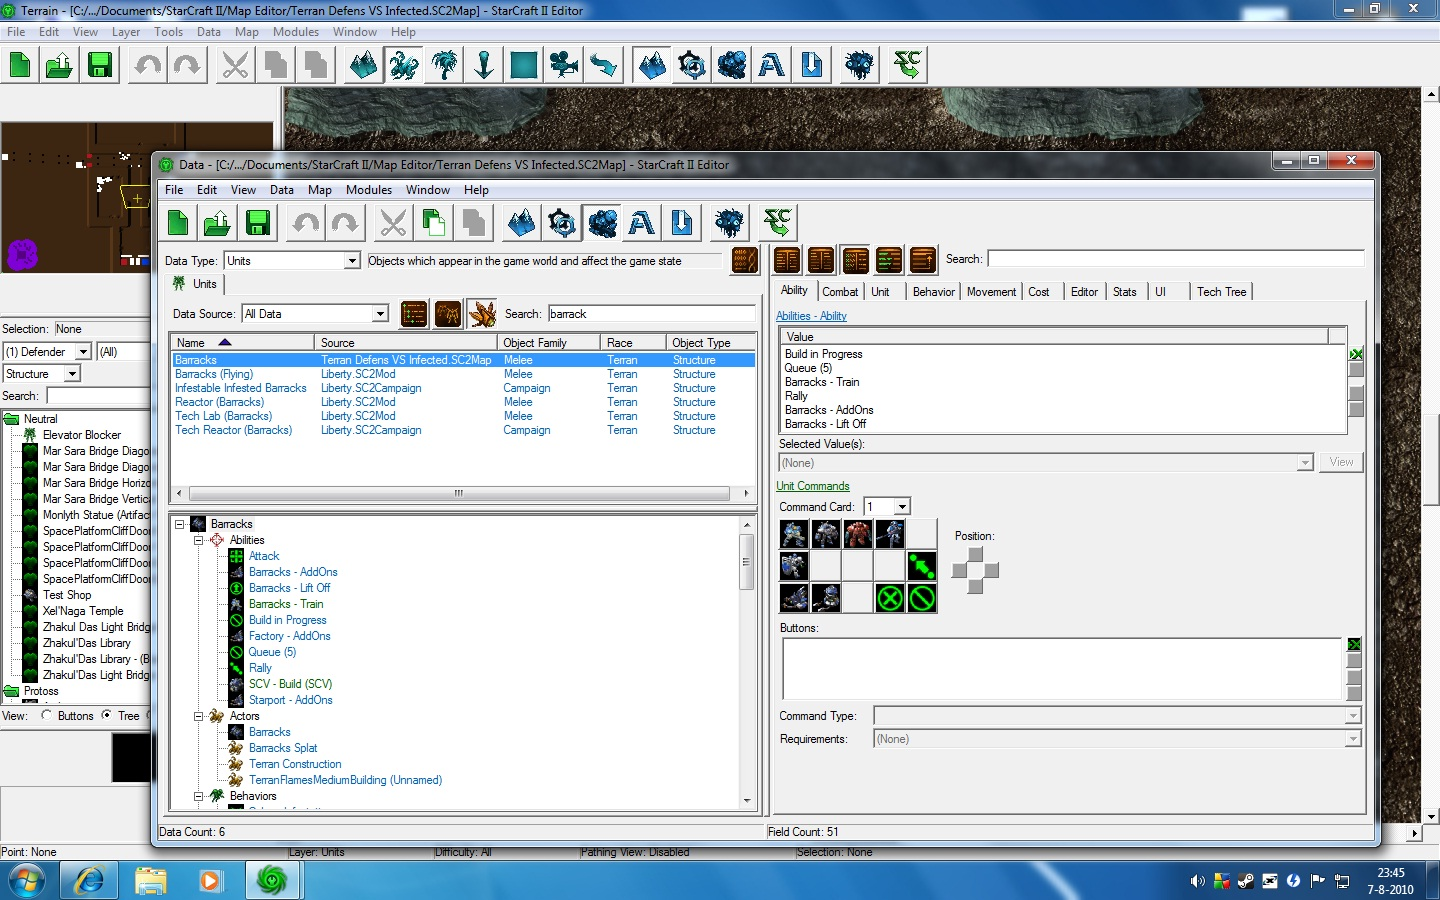
\includegraphics[width=10cm]{../img/sc_editor.jpg}
    \caption{Besides map editing, some editors -- like the Starcraft editor in this figure -- can be used to edit entities.
             \\Source: \href{http://www.darvo.org/images/Tutorials\%20Starcraft\%202/Adding\%20Units\%20to\%20a\%20Building\%20part\%201.jpg}
             {http://www.darvo.org}}
    \label{sc-editor}
\end{figure}

While this approach could be easily implemented using configuration files for entities, our goal \textbf{(G2.1)} requires the ability
to alter the behavior of entities which includes creating entirely new behavior and thus only selecting predefined AI won't suffice.
To achieve this, we could require our users to write the behavior using a scripting language, which wouldn't be much different
from the previous option. Alternatively, we could create a graphical tool that would allow the user construct the behavior out of blocks
representing decisions and actions which would then be translated to source code -- again, requiring a scripting language interfaced
to the engine. An example of such graphical tool is the blueprint system used by Unreal Engine~\cite{UE}.

\begin{figure}[h]
    \centering
    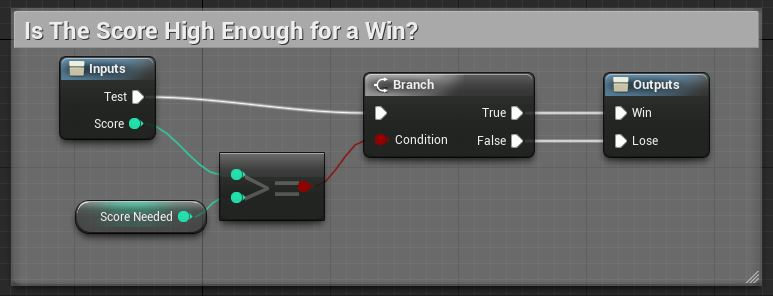
\includegraphics[width=10cm]{../img/blueprints.jpg}
    \caption{A simple blueprint checks if a person passes a test.
             \\Source: \href{://docs.unrealengine.com/latest/images/Engine/Blueprints/UserGuide/Macros/score\_comparison\_example\_macro.jpg}
             {http://www.unrealengine.com}}
    \label{ue-blueprints}
\end{figure}

In Figure~\ref{ue-blueprints} we can see an example blueprint created in Unreal Engine, it comprises interconnected blocks that represent
conditions, loops, actions and other constructs that can be found in a typical programming language. The user uses these blocks to
create programs in a more user friendly manner. Unreal Engine then uses these blueprints to generate C++ code that is then used in the game.

Since we want the mods for our game to be easy to create, implementing an editor would be ideal as it would open modding to an even
broader audience. But implementing a system that is similar to Unreal Engine's blueprints would be far out of the scope of this thesis,
though it might be a good future addition to the project.

\section{Programming Language}

The first tool we need to decide on is the programming language we are going to write our game in.
This choice affects multiple aspects of the final game. These aspects can include, but are not limited to:

\begin{itemize}
    \item Performance: Interpreted languages tend to be slower than compiled languages, but this
        does not to be always true due to the existence of Just-In-Time -- often abbreviated as \emph{JIT} -- compilers, 
        which can provide compilation
        to machine language at program start and runtime optimizations to increase the performance.
    \item Speed of development: Lower level languages often require the implementation of tools that
        are provided by the standard libraries of higher level languages.
    \item Modifiability: Some programming languages -- e.g. interpreted ones -- provide means to
        alter the source code at runtime, while other require recompilation or the use of an embedded language.
\end{itemize}

The programming language that will be used to create our game needs to have one or more libraries that will allow us
to create 3D graphics and be fast enough to offer at least the minimum acceptable framerate while rendering game objects
to the screen, updating the state of the game and processing user input. It should also allow our players to modify the game
even if they only have the distributed version of the game -- meaning it should be able to load code it was not originally compiled
with.

Since mod development requires testing of the mod's functionality in the game, it would be beneficial if the game allowed
our mod creators to change the game's mechanics and data at runtime so that they do not need to restart the game
to see what effect does a change in their mod have on the game. This means that the ability to execute a piece of code
input as a string or load source files during runtime is a feature our programming language should provide.
Lastly, the language should allow us to create a modding API that can be provided to our users as discussed in the previous section.

Aside from these important characteristics, the language should also be easy to use by those of our players that decide to
modify the game.

\subsection{Native Language: C++}

C++, the first language we are going to look at and also the language we ended up choosing, was for a long time the
industry standard when it comes to video games. One of the main reasons for this was that it is -- unlike some of its
rivals, e.g. C\# or Java -- a language that is native, i.e. compiles directly into machine code of a specific processor, 
which generally results into faster executed code.

This benefit of the language, while still present, got weakened by the rise of JIT compilers as both C\# and Java can now
compile their intermediate language the first time it's executed. Since by the time this compilation takes place the
compiler knows what operating system, architecture and hardware specification it compiles for it can provide optimization that
a C++ compiler cannot perform, achieving comparable execution speeds.

Even though the performance gap between these languages got reduced, the era of C++ being one of the most used programming languages
in game development has resulted into an abundance of game programming related materials like libraries, tutorials and books.

One of our main requirements for a programming language is the ability to load code it was not originally compiled with. C++ allows this
with the use of dynamically loaded libraries, but this approach is not easy to use by our mod creators as they would be required to
directly interface their mods with the C++ code of the game's engine. An alternative to this approach is to use more user friendly
language embedded into C++ -- e.g. Lua -- and handle the interface between C++ and this language ourselves. This option also
allows the execution of a code input to the game at runtime, which satisfies another of our requirements.

The reason we decided to choose C++ as the language our game is going to be written in is mainly a combination of the abundance of
various game development related resources aimed at C++ -- be it books, tutorials or even answered questions that can be found
on internet -- and the author's knowledge of the language.

\subsection{Managed Languages: Java and C\#}

Managed languages, unlike native ones such as C++, are compiled to an intermediate language which can then either
be interpreted by a virtual machine or JIT compiled into machine code of the target architecture. The use
of a JIT compiler allows execution speeds that are comparable to those of C++.

Where they beat C++ is in their approachability, as they abstract memory management and other lower level aspects of programming
from the programmer. As such, use of these languages would lead to an easier mod making process for our players, but as
we have already settled in the previous section, that can be done in C++ using an embedded language with easier to
understand syntax and semantics.

Both of the managed languages that were taken into consideration -- Java and C\# -- provide an easy way to execute code input
at runtime using either the Java Compiler API~\cite{JavaCompAPI} or the Roslyn sompiler service~\cite{Roslyn} available in C\#.
Alongside this feature both languages offer the ability to embedd another language throu the use of libraries such as
LuaJ~\cite{LuaJ} or NLua~\cite{NLua}.

The difference of these two languages lies in their environment. The Java Virtual Machine -- often abbreviated as JVM -- provides
the ability to compile the code once and then run the resulting executable file anywhere, which can be beneficial for an ordinary
desktop application. When it comes to games, this advantage loses part of its strength due to the fact that the majority of the
players use a Windows operating system -- as can be seen in the Steam hardware and software survey~\cite{SteamHW}. According
to the survey, over 95\% of the players that use the Steam platform  play their video games on a Windows system -- ranging
from Windows XP to Windows 10. In this case, the use of a virtual machine -- be it JVM or .NET's Common Language Runtime -- brings
little to no advantage over a native language such as C++ in terms of portability. On the other hand, Java gains a disadvantage
compared to C\# as it requires the player to have the JVM installed, which is not installed on any of these operating systems
by default. This means that our game would require the installation of a third party software -- though the JVM can be bundled
with the distributed game, it would still ask our players to install updates. The necessity of having the .NET platform
installed is not a problem as it is developed by Microsoft,
which is also the developer of the Windows operating systems, and as such can be installed through Windows and automatically kept
up to date by the Windows Update service.

Because of this problem, the Java programming language was not chosen for the implementation of our game. C\#, on the other hand,
is an easier to use language than C++ and offers the ability to be modded in itself. Being able to have our game to be modded
in C\# would be beneficial seeing as the Unity3D game engine~\cite{Unity} uses it for scripting and thus many game developers
and modders are already capable of using it. Considering these characteristics of the language, we find it to be equal -- if not
superior -- to C++ in terms of game development capability. The reason for not choosing C\# as the language to write our game in
was the fact that the author has more experience with C++.

\section{Scripting Language}

Now that we have chosen C++ as the programming language we are going to implement the engine of our game with, we need
to choose which language we are provide our modding interface in. Such a language should be easily embeddable within C++,
easy to use and well known in the modding community so that people with modding experience can easily create mods for our game.

\subsection{Lua}

Lua is a programming language that was designed to be embedded into other languages like C or C++ and as such
provides a simple to use API written in ANSI C allowing easy function
binding and data sharing between C/C++ and Lua. These characteristics, along with others such as small memory
footprint, easy to understand syntax and
high configurability using provided meta mechanisms, caused Lua to become the most favorite language used for game 
scripting~\cite{EngineSurvey}.

Due to the high amount of games using Lua for scripting -- e.g. the Wikipedia category called "Lua scripted video games" contains
157 entries~\cite{LuaScriptedVGs} -- there is already a large amount of mod creators that know how to use the language to
create mods for games and as such the use of Lua in our game would make our modding tools more familiar to players that already have
experience in modding.

The ability to easily embedd Lua to our engine written in C++ along with the familiarity the modding community already has with the
language were the main reasons for choosing Lua as the scripting language for our game.

\subsection{Python}

While Python is similar to Lua with its easy to understand syntax, its ability to be embedded to C++ is bit worse in comparison.
The various C++/Python interface APIs are mostly designed to allow the extension of Python using C++ and as such require more
work to embedd Python in C++ -- e.g. unlike Lua, which uses a special stack to communicate with C++, the CPython API~\cite{CPython}
requires manual reference decrementing and incrementing for heap allocated Python objects used in C++.

Where Python generally beats Lua is the abundance of libraries it has available, ranging from scientific libraries to image manipulation
libraries. But since our scripting language will be mainly be used as an interface to the functionality of our engine, these libraries
offer little to no advantage over Lua's minimalistic standard library.

The main downside of using Python as our scripting language is in the fact that Lua is used more often as a scripting language in games
-- the Wikipedia category called "Python scripted video games" contains 17 entries~\cite{PythonScriptedVGs}, which is much lower
than Lua's 157 entries. This means that the modding community will probably not be used to writing mods in Python as much as they are
in Lua. This downside, along with the significant whitespace Python uses -- which might be a bit confusing to a non-programmer that
would want to mod our game -- were the main reasons for choosing Lua over Python.

\subsection{AngelScript}

AngelScript~\cite{AngelScript}, similarly to Lua, is a programming language designed to be embedded into other languages for scripting.
The main advantage it has over Lua is that it is even easier to embedd within C++ because of its C++-like design, requiring only
a simple registration of C++ functions in order to be able to call them.

This advantage is also the main downside of the language, as its C++-like syntax is not as easy to understand as Lua's. This means that while
AngelScript would be easier to embedd into the engine, the modding API wouldn't be as begginer friendly as if it were interfaced
to Lua. Because of this downside and a smaller amount of games that use -- according to the official website~\cite{AngelScriptGames}, 
only 35 games use AngelScript for scripting -- we have decided to choose Lua over AngelScript.

\section{Entity Representation}

In this section, we are going to investigate different approaches for entity representation in our engine, that is, how is each
entity -- i.e. anything that is part of the game world, such as a minion, a wall, a trigger, a task or an event -- will be
structurally represented in our engine. This includes the entity's data, logic and relationships between different entities.

Since our goal \textbf{(G2.1)} requires easy modification of entities, our requirements for the entity representation are:
\begin{itemize}
    \item Extensibility: It should allow easy addition of new entity types so that mods can define new entities for their mods. It
        should, if possible, also allow this extensibility at runtime, which would provide means for easy runtime testing and prototyping.
    \item Modifiability: It should allow easy modification of predefined entity types so that mods can change entities that are already
        present in the unmodded game.
    \item Performance: Since the entity updating will, along with rendering, take the majority of execution time, the representation should
        allow fast entity updates.
    \item Ease of Lua binding: It should be easily representable in Lua even if the entities are defined in the C++ engine.
\end{itemize}

After taking these requirements into account, we decided to choose the Entity Component System representation
-- often abbreviated as \emph{ECS} -- over
the alternatives -- inheritance based and Entity Component representations.

\bigskip
Ask PJ: The term representation -- does it sound OK? It basically means how an entity is structured/represented within the engine
and I wasn't able to come up with a more suitable term.

\subsection{Entity Component System}

Entity Component System is a structural design pattern that endulges the \emph{composition over inheritance} principle.
It comprises three main elements: \textbf{Entity}, \textbf{Component} and \textbf{System}.

\begin{itemize}
    \item Entity is an identifier of anything that is present in the game world. It can be as simple as a numeric 
        identifier or a more complex object, such as a component container.
    \item Component is a piece of logically related data, it generally represents a single characteristic 
        of an entity, such as its health, position, collision box, movement or behavior.
    \item System updates a single component or a set of components of all entities that have these components.
\end{itemize}

\begin{figure}[h]
    \centering
    \begin{lstlisting}[frame=single]
        entity = {
            health_component = {
                health = 50,
                max    = 100,
                regen  = 2
            }
        }

        health_system = {
            components = { entity.health_component },

            function update()
                for comp in components do
                    if comp.health < comp.max then
                        regenerate(comp)
                    end
                end
            end,

            function regenerate(comp)
                regenerated = comp.health + comp.regen
                comp.health = min(comp.max, regenerated)
            end
        }
    \end{lstlisting}
    \caption{A simple health system that regenerates the health of every entity
            that has a health component.}
    \label{ecs-example}
\end{figure}

In Figure~\ref{ecs-example}, we can see an example of a system that -- on a set period -- regenerates the health of all entities
that have a health component. The \emph{health\_system} iterates over all \emph{health\_components}, which contains all
data related to health and regeneration. Updating the game state in ECS is then done by updating all systems.

This representation satisfies all of our three requirements. Since entities are nothing but a set of components, we can specify
which types of components constitute an entity in a simple script and we can even create completely new types of entities
during runtime by creating a new identifier and assigning components to it.

Similarly, we can add new components and remove existing components of an entity, which allows modification of already existing
entities. As an example, we can add a movement component to a stationary entity to make it able to move. This, like the definition
of new entities, can be easily done at runtime.

An interesting characteristic of the ECS is its satisfiability of our last goal -- performance.

% TODO
\begin{itemize}
    \item define the ECS design pattern
    \item mention how well it supports run time entity creation and modification
    \item mention ease of development this model creates
    \item mention ease of entity access (through ID)
    \item talk about the difference between Component and ECS patterns
    \item ?mention cache friendliness? (pro: well, it exists, con: not used that
        much in this game)
\end{itemize}

\subsection{Inheritance}

% TODO
\begin{itemize}
    \item explain what is meant by the title (classic OOP design)
    \item this kind of engine would also have to be planned a lot (to avoid
        inheritance hierarchy hell)
    \item ?say that it's not as performant as the other two?
\end{itemize}

\subsection{Entity Component}

% TODO
\begin{itemize}
    \item define the Component design pattern (with references to
         the gamedesginpatterns.smth book)
    \item mention that this is very similar to the component based implementation
         both Unity and UE4 use
    \item mention its relationship with both ECS and the inheritance based design
\end{itemize}

\iffalse

\section{Libraries}

% TODO
\begin{itemize}
    \item just mention something about reinventing the wheel and
        the areas for which 3rd party libraries were used
\end{itemize}

\subsection{3D Rendering}

TODO: Merge OpenGL and DirectX together as low level API and add more high level libs.
% TODO
\begin{itemize}
    \item almost any game will have to use some library for this as
        going without would take years
    \item ??I only though about these in the beggining, should I add
        others just for comparison??
    \item mention that portability of the rendering library is much more
        important than for example the GUI library, since it's integrated
        deep into the engine while the GUI is not
\end{itemize}

\subsubsection{OpenGL}

% TODO
\begin{itemize}
    \item talk about what it is
    \item would allow later Linux port
    \item too low level, would slow the development process
\end{itemize}

\subsubsection{DirectX}

% TODO
\begin{itemize}
    \item talk about what it is
    \item similar problem to OpenGL (too low level)
    \item would prohibit eventual port to Linux
\end{itemize}

\subsubsection{Ogre3D}

% TODO
\begin{itemize}
    \item talk about what it is
    \item can wrap both OpenGL and DirectX
    \item higher level, lots of stuff already implemented
    \item describe basic usage of the library (entities, meshes, scene graph, ...) 
\end{itemize}

\subsection{Graphical User Interface}

% TODO
\begin{itemize}
    \item main requirement is Ogre compatibility
    \item theoretically does not have to be portable as it can easily be changed
        (as it's not integrated into the engine)
    \item other requirements: graphical editor, ease of use, high level, all the
        widgets needed (buttons, scrollbars, editboxes, labels, ...)

\end{itemize}

\subsubsection{Ogre Overlay}

% TODO
\begin{itemize}
    \item talk about what it is
    \item too simple, would require for the widgets to be created during
        the game development process which would take a lot of time
\end{itemize}

\subsubsection{CEGUI}

% TODO
\begin{itemize}
    \item talk about what it is
    \item used to be bundled with Ogre
    \item easy to use, clean interface, good design
    \item ??? genrally advised by the Ogre community
    \item ??? used for Torchlight which proved what can be done with it
    \item graphical editor and existing skins
    \item ??I only though about these in the beggining, should I add
        others just for comparison??
\end{itemize}

\section{Algorithms}

% TODO
\begin{itemize}
    \item dunno about this section, not many known or big
        algorithms used in the game
\end{itemize}

\subsection{Pathfinding}

% TODO
\begin{itemize}
    \item talk about the problem of pathfinding
    \item talk about node graph vs vertex graph (or hows it called)???
    \item after mentioning node graph, give reason for grid form
	    and 8 neighbours (bcuz of the view)
    \item also talk about the inclusion of portals in pathfinding
	    and problems that have risen with it
\end{itemize}

\subsubsection{Breadth-first Search}

% TODO
\begin{itemize}
    \item just mention what it is and why it's not good
	    (uniform cost of graph edges)
\end{itemize}

\subsubsection{Dijkstra}

% TODO
\begin{itemize}
    \item talk about what it is and why it's not the best alternative
    \item explain that it might be worth using when performance is
	    not critical and we absolutely need the best path
\end{itemize}

\subsubsection{A*}

% TODO
\begin{itemize}
	\item talk about what it is (possibly also define heuristic as it should
		be seen for the first time now)
	\item mention that it's probably the most used one in games (provide examples?)
	\item ??mention how it goes well with e.g. portals??
	\item maybe go into detail about the default heuristic (PORTAL\_HEURISTIC) which
		allows portal pathfinding (include previous iterations, portal component,
		problem with portal chains and possible fix)
\end{itemize}

\subsubsection{Solution ??}

% TODO
\begin{itemize}
    \item maybe this should be in the A* part as it's the only one actually implemented?
    \item describe the generic pathfinding system implemented in the game, switchable
	    algorithms, heuristics and path types (define path type),
	    algorithm and path type interface ...
\end{itemize}

\section{Serialization}

% TODO
\begin{itemize}
    \item talk a bit about game state serialization in general
    \item mention that since the game should be extensible, manual save game
	    editing without the need to write big editors would be nice
	    for testing and possibly the creation of simple mod maps
	    (and the save editor - if ever created - would be easy to make)
\end{itemize}

\subsection{Binary}

% TODO
\begin{itemize}
    \item mention that it's the most used
	    (maybe give examples like UE4 save system etc.)
    \item it's also the most compact as it just meshes data together in binary
    \item lots of libraries (like boost)
    \item editing would require complex editor and does not allow code execution in the
	    save file so additional save file functionality (like changing the wave
	    system table, executing custom commands) would need to be made in C++
	    in a generic way, which would be bad for mods
\end{itemize}

\subsection{XML}

% TODO
\begin{itemize}
    \item mention losts of xml libraries
    \item talk about how it allows easy data change, which in a data driven game like this
	    one means quite a lot
    \item but explain that it's bad because it disallows code execution
\end{itemize}

\subsection{Lua}

% TODO
\begin{itemize}
    \item since the game needs an extensive modding api with all sorts of setters/getters,
	    all that's needed is to write serialization of components into a sequence of
	    the API calls
    \item easy to implement, load is basically executing a script
    \item easy to modify using a text editor
    \item !!allows code execution to create special levels
    \item say that it's limitation is level size, e.g. 256x256 save file can be big (200MB) and
	    very slow to load (10-20sec), but on the allowed level sizes (10-64) the load
	    is almost instant and the resulting files small (16x16 is around 650KB)
\end{itemize}

\section{Levels}

Addition: Talk about level representation and how using the same
format for saved games and levels helps the creation of custom maps.

% TODO
\begin{itemize}
    \item talk about how complex level generation isn't really needed due
	    to the nature of the game (you dig your own hallways so only need
	    gold distribution)
    \item mention that similar generic system to the pathfinding one is used
    \item ??probably go through the algorithm in pseudocode?? or explain it only??
	    if so, probably go through the part with the gold only and just mention
	    the rest??
\end{itemize}

\section{Spells}

Here just compare the original idea of having the spell system in C++ and the current version
of defining spells fully in lua and C++ just call callbacks basically.

\fi
